
\section{ʵ������}
\label{sec:heart_experiments}

\subsection{ԭʼ������ʵ������}
\label{subsec:heart_setup_data}

Considering our aim and the requirements on the computation resources, the volume containing the whole heart was extracted from the original one that include the whole body trunk of an anonymous patient. %
The dataset, in resolution of $0.4\text{mm} \times 0.4\text{mm} \times 0.6\text{mm}$, was acquired on a 128-slice CT modality (Siemens SOMATOM Definition Flash).

Numbers of experimental trials were carried out on the image dataset, applying distinct sets of parameters for the evaluation of the approach.
%In our case, the CTA series in DICOM format had been converted to the form of XML first.
%Then the converted data was fed into the feature image production branch and input level sets generation branch.
%The resulting data from the two branches were sent to geodesic active contours module in order to generate the final results.
%Finally, the marching cubes method is used to visualize the segmented data.
The experiments were executed on a desktop machine armed with Intel's 2.83GHz Core 2 Quad CPU and 4GB RAM.

\subsection{Ԥ����}
\label{subsec:heart_preprocessing_experiments}

As mentioned in Sec. \ref{subsec:heart_overview}, series of preprocessing were conducted before the evolution of the ``snakes":
(i) the image smoothing preserving the edges;
(ii) the exclusion of the uninterested image details;
(iii) the calculation of the image gradient magnitude;
(iv) the generation of the initial contours.

As the first step, an algorithm based on MCDE given by (\ref{eqn:heart_MCDE}) was utilized to smooth the input images.
By applying this numerical method, the edges in the images were well protected from the smoothing effect.

Then the binary thresholding was applied in order to exclude most uninteresting contents, i.e., only the contents of interest were left after this step.
In achieving this goal, the properly chosen threshold pairs (i.e., the lower and upper thresholds) were decided based on the analysis of the histogram of the smoothed images.
The ``useful" contents were highlighted as bright intensities (i.e., $255$ for the binary thresholding), whilst the unwanted contents were all assigned to zero.
Figure \ref{fig:heart_binary_threshold_experiments} depicted the results of the binary thresholding step.
\begin{figure}[t]
\centering
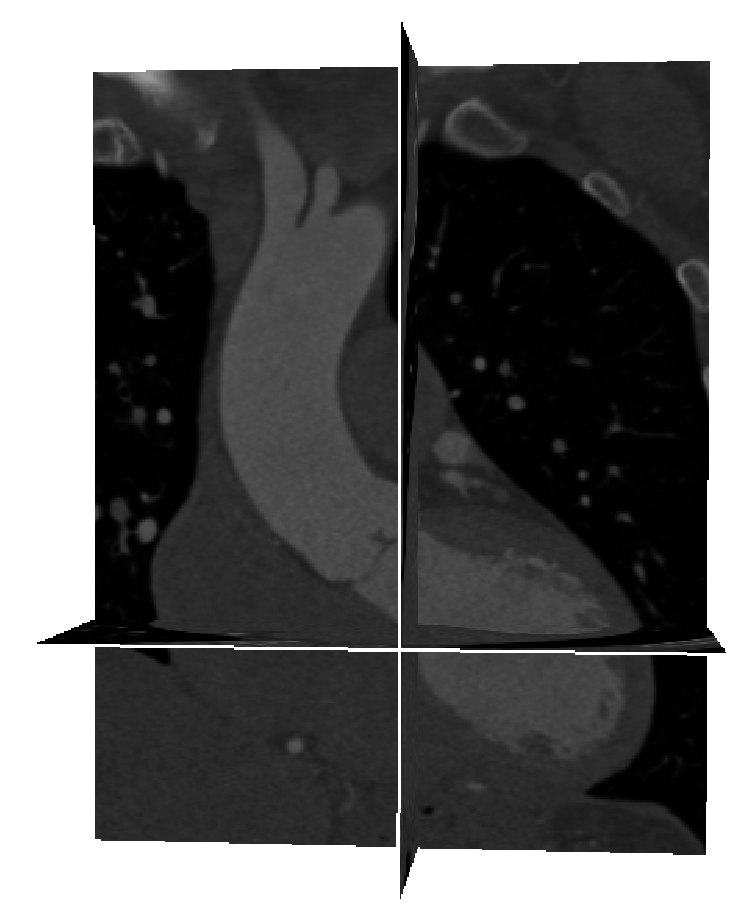
\includegraphics[height=2.6in]{Figures/heart/original.eps}
\caption{The anterior view of the original volume contains the whole heart region extracted from the raw CT image series acquired from a real patient.}
\label{fig:heart_original}
\end{figure}
\begin{figure}[t]
\centering
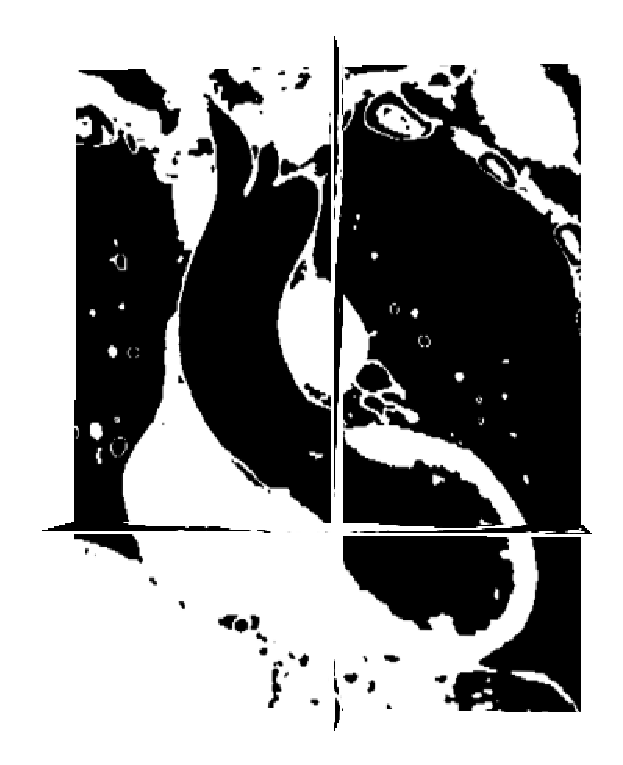
\includegraphics[height=2.6in]{Figures/heart/binary_threshold.eps}
\caption{Volume after the binary threshold processing. Note that the pericardium, and most of the blood vessel structures are excluded.}%
\label{fig:heart_binary_threshold_experiments}
\end{figure}

\subsection{Calculation of Gradients and Initial Contours}

After thresholding the images into the binary form, the rest two steps (the calculation of the edge potential and the initial contours) were performed simultaneously.
The aim of pixel-wisely computing of the gradients is to provide the ``snakes" model the references of the edges of the objects.
As a matter of fact, the reference images were generated by applying the nonlinear intensity mapping after the computation of the gradients.
On the other hand, the initial contours were evolved by applying the fast marching algorithm \cite{Sethian1999} for the purpose of providing the ``snakes" the distance information of the images. %
The resultant images included the time-of-arrival (i.e., in the form of the intensity value) of the evolving fronts at each pixel.

\subsubsection{Computing the Gradients}

In calculating the edge potential of the images, the work was divided into two consecutive steps:
Firstly, the gradient magnitude of the images were calculated by solving (\ref{eqn:heart_gaussian}).
Secondly, the results of the previous step were converted into the appearance that the edges are dark while the rest of the images are bright.
The S-shape function defined by (\ref{eqn:heart_sigmoid}) has four parameters to control the window width $m$, the window location $n$, and the extreme values $\alpha$ and $\beta$ of the intensities in the output images.
Figure \ref{fig:heart_sigmoid_width} shows how to control the window width by adjusting the parameter $m$.
The larger the absolute value of $m$, the wider the window; while the minus sign indicates that the inversion of the pixels.
Figure \ref{fig:heart_sigmoid_center} shows how to control the window location by adjusting the parameter $n$.
The larger the absolute value of $n$, the further the center of the window away from the origin.
The minus sign indicates that the window shift left; otherwise shift right.
In converting the gradient images, the selection of the parameters $m$ and $n$ were essential.
Their values depended the two extreme intensities of the pixels in the gradient images.
In the experiments, the guideline of the selection was: $m < 0$, and $n > 0$, where $n > |m|$.
The resultant images demonstrated the edges of the objects in zero intensity ($\alpha = 0$) while the inside/outside areas in the maximum intensity (i.e., $\beta = 255$).
\begin{figure}[t]
\centering
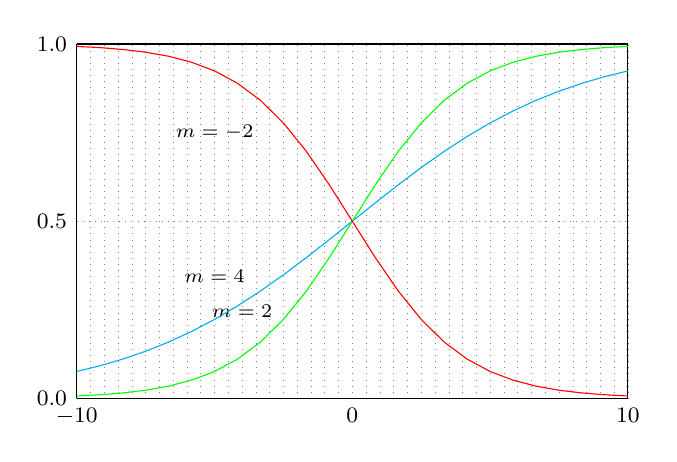
\begin{tikzpicture}[xscale=0.35,yscale=4.5]
\draw [help lines,dotted,step=0.5] (-10,0) grid (10,1);
\draw [thin] (-10,0) -- (-10,1);
\draw [thin] (-10,1) -- (10,1);
\draw [thin] (10,0) -- (10,1);
\draw [thin] (-10,0) -- (10,0);
\node [below] at (0,0) {\footnotesize{$0$}};
\node [left] at (-10,0) {\footnotesize{$0.0$}};
\node [left] at (-10,0.5) {\footnotesize{$0.5$}};
\node [left] at (-10,1) {\footnotesize{$1.0$}};
\node [below] at (-10,0) {\footnotesize{$-10$}};
\node [below] at (10,0) {\footnotesize{$10$}};
\node [below] at (-5,0.8) {\scriptsize{$m = - 2$}};
\node [above] at (-5,0.3) {\scriptsize{$m = 4$}};
\node [above] at (-4,0.2) {\scriptsize{$m = 2$}};
\draw [cyan,thin,domain=-10:10] plot (\x,{1/(1+exp(-0.25*\x))});
\draw [green,thin,domain=-10:10] plot (\x,{1/(1+exp(-0.5*\x))});
\draw [red,thin,domain=-10:10] plot (\x,{1/(1+exp(0.5*\x))});
\end{tikzpicture} 
\caption{Relation between the parameter $m$ and the window width of the S-shaped function for nonlinear intensity mapping: the curve with $m = 4$ (in cyan) can invert the pixels lie between wider range than the ones with $m = -2$ (in red) and $m = 2$ (in green). Note that the minus sign of $m$ can introduce inverse effect to the output.}%
\label{fig:heart_sigmoid_width}
\end{figure}
\begin{figure}[t]
\centering
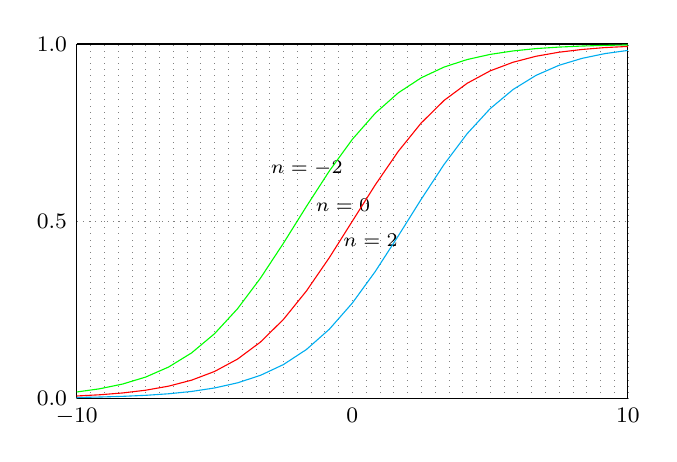
\begin{tikzpicture}[xscale=0.35,yscale=4.5]
\draw [help lines,dotted,step=0.5] (-10,0) grid (10,1);
\draw [thin] (-10,0) -- (-10,1);
\draw [thin] (-10,1) -- (10,1);
\draw [thin] (10,0) -- (10,1);
\draw [thin] (-10,0) -- (10,0);
\node [below] at (0,0) {\footnotesize{$0$}};
\node [left] at (-10,0) {\footnotesize{$0.0$}};
\node [left] at (-10,0.5) {\footnotesize{$0.5$}};
\node [left] at (-10,1) {\footnotesize{$1.0$}};
\node [below] at (-10,0) {\footnotesize{$-10$}};
\node [below] at (10,0) {\footnotesize{$10$}};
\node [above left] at (2,0.4) {\scriptsize{$n = 2$}};
\node [above left] at (0,0.6) {\scriptsize{$n = - 2$}};
\node [above left] at (1,0.5) {\scriptsize{$n = 0$}};
\draw [cyan,thin,domain=-10:10] plot (\x,{1/(1+exp(-0.5*(\x-2)))});
\draw [green,thin,domain=-10:10] plot (\x,{1/(1+exp(-0.5*(\x+2)))});
\draw [red,thin,domain=-10:10] plot (\x,{1/(1+exp(-0.5*\x))});
\end{tikzpicture} 
\caption{Relation between the parameter $n$ and the location of the center of the window of the S-shaped function for nonlinear intensity mapping: the curve shifts right when $n < 0$ (e.g., the curve in green), and shifts left when $n > 0$ (e.g., the curve in cyan). Note that the absolute values of $n$ regulate the distance from the origin.}%
\label{fig:heart_sigmoid_center}
\end{figure}

\subsubsection{Evolving the Initial Contours}

Meanwhile, the evolution, driven by the fast marching algorithm \cite{Sethian1999}, started with the aim of generating the initial contours for the geodesic ``snakes" computation.
The results provided the geodesic computation the \emph{time-crossing} map so that the ``snakes" can evolve according to the computed time-of-arrival.
In this step, the only human intervention was the selection of the input seeding points, from which the computation would begin.
The location of the seeds should be located interior of the targets, and the sign of the speed function $F$ in (\ref{eqn:heart_Eikonal}) should be positive to ensure outwards propagation of the contours. %

\subsection{���ѧ�������ˮƽ���ݽ�}
\label{subsec:heart_geodesic_experiments}

The evolution of the geodesic ``snakes" started from the seeding points fed in previous step for the generation of the initial contours.
The ``snakes" utilized the resultant initial contours as the map in which all the pixels were marked with the time when the fronts ever crossed them.
On the other hand, that edge potential maps depicted the general geometric feature of the images, in which the magnitudes of the gradients were calculated and represented to show the ``valleys" and the ``plains" in the images. %

In order to speed up the calculation, sufficient ``attraction" in (\ref{eqn:heart_geodesic_driver}) was required.
Besides, the disturbance of the false edges during the evolution can be avoided due to larger attraction.
In this work, the original contours were located inside of the targets, meaning that they evolved ``outwards" towards the edges.
During the computation, the speed of the propagation was fast on the ``plains" (i.e., the inner areas of the targets), and was pretty slow when falling into the ``valleys" (i.e., the edges of the targets). %
To terminate the computation in time, the numbers of the iterations was set to $500$ in the experiments.
\begin{figure}[t]
\centering
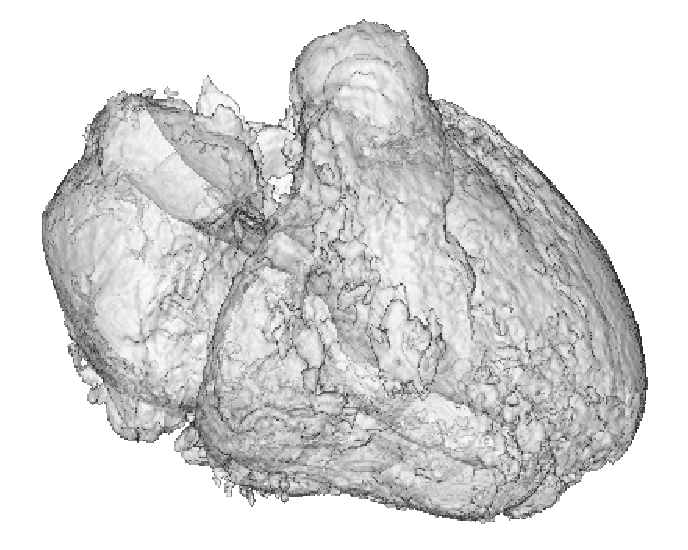
\includegraphics[height=2.4in]{figures/heart/heart.eps}
\caption{The anterior view of the three-dimensional surface model of the heart.}
\label{fig:heart_Heart}
\end{figure}
